\chapter{OpenSITEM: Sistema Federado de Aplicaciones para la Caracterización de Nodos Potenciales de Redes de e-salud}

\textbf{OpenSITEM }es un sistema federado de aplicaciones de software libre o de código abierto que provee herramientas para analizar datos e información de los siguientes elementos que son de interés para la descripción - y definición de capacidad de, nodos potenciales de redes de e-salud: entidades de salud, servicios médicos, tecnologías de interconexión, operadores de telecomunicaciones, equipos médicos, organizaciones, profesionales, estándares, pacientes, enfermedades, medicamentos y proyectos. Provee un ambiente para apoyar las tareas de las comunidades de práctica involucradas en la investigación, el diseño, mantenimiento, desarrollo e implementación de redes de eSalud. Tuvo su génesis conceptual en la primera fase del Proyecto Telemedicina Bogotá como solución a la necesidad de administrar los resultados del estudio de campo realizado a las entidades e instituciones de salud y los operadores de Telecomunicaciones en la ciudad de Bogotá.

Su principal objetivo es: Implementar un sistema que permita la definición, categorización y caracterización de nodos potenciales de redes de eSalud, para apoyar las actividades básicas de los \textit{trabajadores del conocimiento} en el área de la telemedicina del grupo GITEM\footnote{Conformado por profesionales y estudiantes de la Universidad Distrital así como por profesionales de las diferentes instituciones que han participado en los diferentes estudios de campo.}  ofreciéndoles, además de un repositorio de datos, herramientas que facilitan las tareas de capturar, extraer, organizar, analizar, encontrar, sintetizar, distribuir y compartir información y conocimiento de nodos potenciales de las redes de eSalud. OpenSITEM cuenta con herramientas para poder  actualizar el estado de los nodos definods en el modelo base así como para la definición de nodos y categorías inéditas del Sistema de Salud de Bogotá Distrito Capital. El modelo base de nodos y categorías se construye a partir del estudio de campo realizado por el grupo de investigación, haciendo especial énfasis en los requerimientos de eSalud que se definieron en esa época.Con OpenSITEM se sistematiza los resultados de los estudios de campo emprendidos por el grupo de investigación GITEM y se constituye una plataforma para gestionar los datos de nodos potenciales de redes de eSalud. Contribuye a disminuir el tiempo de adquisición, análisis y despliegue de la información.  
\begin{figure}
 \centering
 
\includegraphics[width=142mm, height=190mm]{sitem_principal.png}
 \caption{Imagen en el año 2017 de la página principal de OpenSITEM}
 \label{pantalla_sitem}
\end{figure}

El proceso de integración del sistema\footnote{OpenSITEM es un sistema federado de aplicaciones.} está basado en métodos ampliamente conocidos \cite {balduino2010}, \cite{koch},\cite{jacobson2000},\cite{larman2004}. Para el diseño de los módulos inéditos se ha tenido en consideración principios, patrones y antipatrones, tratando de minimizar los riesgos asociados a la mala calidad del software.

OpenSITEM hace uso extensivo de aplicaciones existentes, marcos de trabajo, bibliotecas, APIs, servicios web y plantillas, lo que ha permitido lograr un alto grado de funcionalidad específica. Los módulos propios\footnote{En referencia a la autoría, no al carácter de código abierto.} - aquellos que hacen parte de la suite desarrollada por GITEM - se implementan sobre el framework OpenSARA \footnote{Diseñado y construido por GITEM. OpenSARA es un producto de este proyecto y se ha usado en otros dominios tanto en la Universidad Distrital (sistema de gestión de inventarios, sistema de consultas a comunidades, sistema de evaluación para acreditación, entre otros), como por algunas empresas del sector TI (OpenKyOS).}.

\section{Módulos Funcionales}

OpenSITEM- incluyendo las aplicaciones de terceros y las desarrolladas por GITEM, ofrece los siguientes módulos base:

\begin{table}[]
\centering
\caption{Módulos base de OpenSITEM}
\label{tabla_modulos_opensitem}
\begin{tabular}{lcl}
\rowcolor[HTML]{C0C0C0} 
\multicolumn{1}{c}{\cellcolor[HTML]{C0C0C0}\textbf{Módulo}} & \textbf{Elaboración} & \multicolumn{1}{c}{\cellcolor[HTML]{C0C0C0}\textbf{Nombre}}            \\
Motor de Federación de Aplicaciones                         & Propia               & OpenSITEM-FE                                                           \\
Motor de recomendación                                      & Propia               & OpenSITEM-RS                                                           \\
Gestión de Nodos                                            & Propia               & OpenSITEM-NM                                                           \\
Diseñador de Redes                                          & Propia               & OpenSITEM-ND                                                           \\
Analizador de Redes                                         & Propia               & OpenSITEM-NA                                                           \\
Gestión de Encuestas                                        & Propia               & OpenSITEM-PM                                                           \\
Inteligencia de Negocio                                     & Tercero              & Knowage                                                                \\
Sistema de Información Geográfica                           & Tercero/Propia       & \begin{tabular}[c]{@{}l@{}}Cesium\\ qGIS\\ Leaflet\end{tabular}        \\
Gestión Documental                                          & Tercero              & Alfresco                                                               \\
Gestión de Reportes                                         & Tercero/Propio       & \begin{tabular}[c]{@{}l@{}}Reportico\\ Varias bibliotecas\end{tabular}
\end{tabular}
\end{table}

\subsection{Características innovadoras de OpenSITEM}


OpenSITEM presenta innovaciones en diferentes dominios:

\begin{itemize}
 \item Dominio de Aplicación: Desarrolla un motor y un proceso para la federación de aplicaciones. 
 \item Dominio de arquitectura: Propone un modelo de arquitectura para nodos en redes de eSalud.
 \item Dominio de utilidad: Implementa una plataforma para soportar flujos de trabajo de investigadores del GITEM. En el mercado no existe una herramienta que de manera unificada cumpliera con el modelo de requerimientos definido.
 \item Dominio social: Tanto el framework (OpenSARA) como los módulos de OpenSITEM están disponibles en repositorios públicos y cobijados por licencia de código abierto. El framework ya se ha utilizado por equipos de trabajo externos al grupo GITEM. Se tiene presupuestado que la fase IV del proyecto (transición) permita que los datos también sean abiertos. 
\end{itemize}


\section{Descripción de la Arquitectura de OpenSITEM}

OpenSITEM es una aplicación federada de arquitectura orientada a servicios, con características como las descritas en {earl2017}. La integración es realizada por un motor que permite el intercambio de mensajes y la sincronización de sesiones entre los diferentes aplicativos federados sin llegar a considerar una arquitectura de Bus de Servicio Empresarial (ESB por sus siglas en inglés)\footnote{Aunque existen ESB de corte empresarial tales como Mule, WSO2, Apache Service Mix o similares, el análisis de utilidad mostró que la mayoría de funcionalidades que ofrecen nunca serían utilizadas y entonces se optó por la simplicidad arquitectónica y evitar la tarea recurrente de configuración y administración del ESB. Ver el anexo \ref{appendix:lista_de_chequeo_ESB}.} 

El presente informe describe la arquitectura general de OpenSITEM y de los módulos inéditos realizados en el marco del proyecto. Las aplicaciones federadas construidas por terceros se abstraen, visibilizando únicamente las interfaces provenientes de las API o de los servicios web de adaptación. 

\subsection{Arquitectura General}

La descripción de la arquitectura sistema (AD) se realiza con base al modelo conceptual definido en \cite{ISO42010}. Dada la extensión de los artefactos, se presentan aquellos apartes de la AD que a juicio de los autores se consideran relevantes para explicar las propiedades fundamentales.

\subsubsection{Interesados e Intereses}

El proyecto considera una aplicación inédita de la cual no se encontró referente de modelo de dominio. En este escenario se vuelve particularmente importante la identificación de los interesados los cuales están enfocados a los investigadores del grupo GITEM que participan en proyectos relacionados con las redes de eSalud, así como expertos en el diseño de redes de telecomunicaciones y de prestación de servicios médicos.

Los mecanismos utilizados para la identificación fueron:

\begin{itemize}
 \item Entrevistas Directas: Realizadas en su mayoría durante la primera iteración de la fase de inicio. Se definió una entrevista base, anexo \ref{appendix:entrevista_posible_interesado}.
 \item Reunión Presencial: De duración fija (30 minutos) y con agenda previa \footnote{La agenda en las reuniones de identificación fue simple. Se buscaba tener una idea de quienes eran los interesados representativos de los diferentes roles que existen en el grupo.}.
 \item Matriz de identificación: En donde se consignaron las evaluaciones de los atributos de liderazgo, poder de decisión, nivel de interés en el proyecto, conocimiento, actitud ante el proyecto (oposición, neutralidad, soporte), procedencia (externa o interna - GITEM, Universidad). 
\end{itemize}

La siguiente tabla muestra el resultado del proceso de identificación:


\begin{table}[]
\centering
\caption{Principales Interesados}
\label{tabla_principales_interesados}
\begin{tabular}{ll}
\multicolumn{1}{c}{\textbf{Interesado}} & \multicolumn{1}{c}{\textbf{Intereses Principales}}                                                                                                                                                                                                                                                                                                                                                                                                                                                                                                                                                                                   \\
Asistente de Investigación Hospital     & \begin{tabular}[c]{@{}l@{}}*  Ingresar y corregir la información recopilada en el estudio de campo.\\ * Elaborar informes a partir de la información ingresada utilizando diferentes filtros y formatos.\\ * Generar una plantilla del informe de investigación que cumpla con los parámetros exigidos por la Universidad.\\ * Registrar las evidencias de las visitas de campo y demás entregables que exige el proyecto.\\ * Gestionar el proyecto de caracterización de los hospitales.\\ * Visualizar geográficamente algunos atributos del hospital (ubicación, zona de influencia, procedencia de pacientes, etc)\end{tabular} \\
Analista en Proyectos eSalud del GITEM  & \begin{tabular}[c]{@{}l@{}}* Analizar la información de diferentes nodos (centros de atención en salud, proveedores de telecomunicaciones, profesionales de salud, pacientes, equipos médicos, servicios médicos, servicios de educación, etc)\\ * Evaluar la potencialidad de los nodos para pertenecer a una red de eSalud.\end{tabular}                                                                                                                                                                                                                                                                                           \\
Diseñador de redes de eSalud            & \begin{tabular}[c]{@{}l@{}}* Diseñar redes de eSalud a partir de la interconexión de nodos de prestadores de salud.\\ * Evaluar la potencialidad de las redes diseñadas.\end{tabular}                                                                                                                                                                                                                                                                                                                                                                                                                                                \\
Experto en nodo                         & \begin{tabular}[c]{@{}l@{}}* Ingresar y corregir información relacionada con el nodo.\\ * Elaborar informes a partir de la información ingresada utilizando diferentes filtros y formatos.\end{tabular}                                                                                                                                                                                                                                                                                                                                                                                                                             
\end{tabular}
\end{table}

\subsubsection{Punto de Vista Estructural}

La estructura de OpenSITEM se presenta principalmente desde tres puntos de vista:

\begin{itemize}
 \item Punto de Vista de Negocio (\ref{punto_negocio}): Con los grupos de actores, roles generales, servicios de negocio y procesos de negocio.
 \item Punto de Vista de Aplicación (\ref{punto_aplicacion}): Con los grupos de Servicios de aplicación y Módulos de Aplicación (federadas y nativas\footnote{Una aplicación federada es aquella que mayormente ha sidos desarrollada por equipos externos, mientas que una aplicación nativa es la que mayormente ha sido desarrollada por integrantes de GITEM.}).
 \item Punto de Vista Infraestructura (\ref{punto_infraestructura}): Con los grupos de Servicio de Infraestructura y Componente de Infraestructura.
\end{itemize}

\begin{figure}
 \centering
 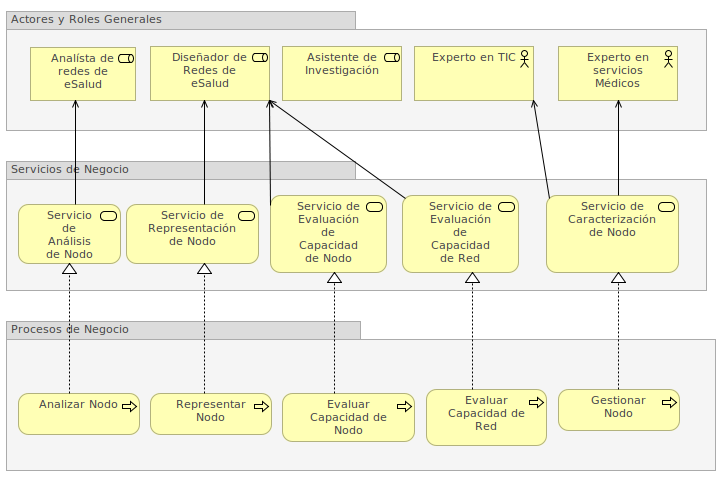
\includegraphics[width=120mm]{negocio_vista_por_capas.png}
 \caption{Punto de Vista de Negocio - Vista Conceptual por Capas}
 \label{punto_negocio}
\end{figure}

\begin{figure}
 \centering
 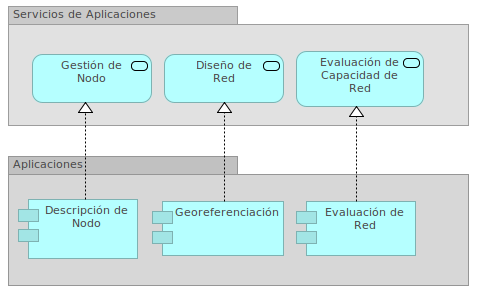
\includegraphics[width=120mm]{punto_aplicacion.png}
 \caption{Punto de Vista de Aplicación - Vista Conceptual por Capas.}
 \label{punto_aplicacion}
\end{figure}

Las aplicaciones nativas se denotan por las iniciales de cada módulo. Por ejemplo el motor de federación (Federation Engine) se conoce como OpenSITEM-FE, el gestor de nodos (Node Management) como OpenSITEM-NM, etc.

\begin{figure}
 \centering
 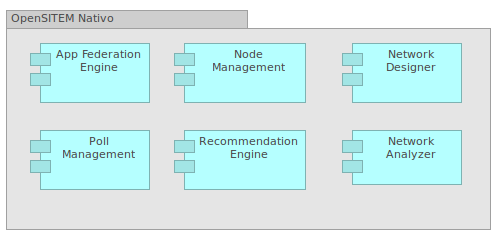
\includegraphics[width=120mm]{opensitem_nativo.png}
 \caption{Punto de Vista de Aplicación - Aplicaciones nativas de OpenSITEM.}
 \label{punto_aplicacion}
\end{figure}


\begin{figure}
 \centering
 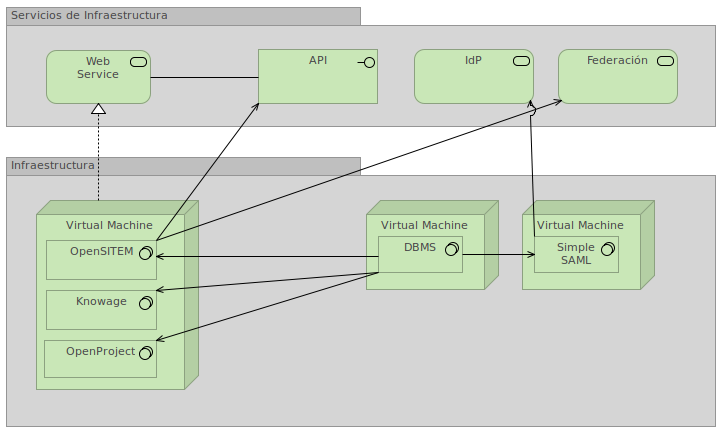
\includegraphics[width=120mm]{punto_infraestructura.png}
 \caption{Punto de Vista de Infraestructura - Vista Conceptual por Capas.}
 \label{punto_infraestructura}
\end{figure}


\subsubsection{Punto de Vista de Comportamiento}

\paragraph{OpenSITEM-FE: Motor de Federación de Aplicaciones}

OpenSITEM no es un sistema de federación universal de aplicaciones. Integra aplicaciones que expongan su funcionalidad a través de interfaz de programación de aplicaciones (API) o de servicios web, utilizando protocolos de la pila TCP/IP con representación basada en XML o JSON. Por esta razón - y por las mostradas en el anexo \ref{appendix:lista_de_chequeo_ESB}; se prescindió de emplear una solución ESB y se diseñó un motor de integración con la siguiente funcionalidad:
\begin{itemize}
 \item Evaluación de Federación: Servicio que se encarga de recibir el mensaje proveniente de una aplicación - a través de un servicio web general, y definir si dicho mensaje hace parte de una transacción que es necesario ser federada. En el contexto de OpenSITEm, se dice que una transacción es federada cuando luego de su ejecución debe ``disparar'' transacciones en uno o varios sistemas diferentes.
 \item Acceso a Aplicación: Servicio por el cual un usuario adquiere las credenciales para acceder o consumir un servicio específico de una aplicación federada.
 \item 	Registro de transacción: Servicio específico por aplicación federada que se encarga de consumir un servicio web, y objetivo es realizar una transacción en una aplicación. 
\end{itemize}

\begin{figure}
 \centering
 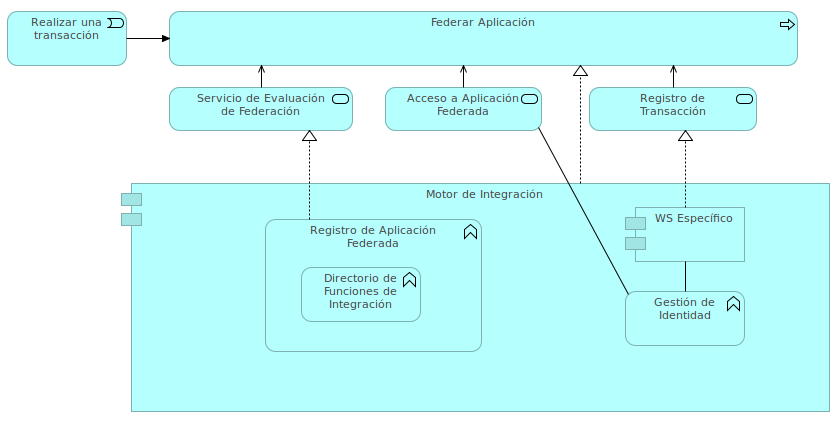
\includegraphics[width=120mm]{motor_integracion_vista_comportamiento.png}
 \caption{Punto de Vista de Comportamiento - Modelo General del Motor de Federación de Aplicaciones.}
 \label{punto_infraestructura}
\end{figure}


\subsubsection{Punto de Vista de Distribución}

Tanto OpenSITEM como cada una de las aplicaciones federadas están desplegadas en una infraestructura virtualizada. Aunque al momento de elaborar este informe se está trabajando en migrar a contenedores, la tecnología que se empela esta 100\% relacionada con máquinas virtuales.

\begin{figure}
 \centering
 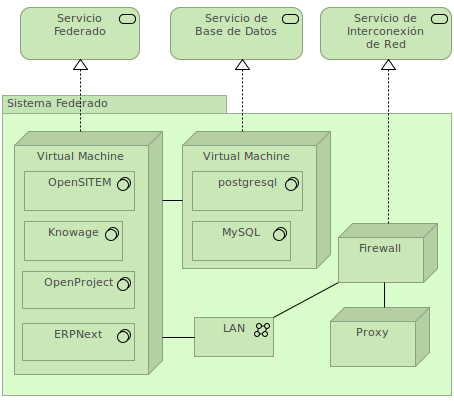
\includegraphics[width=120mm]{openSITEM_Vista_Distribucion.png}
 \caption{Punto de Vista de Distribución.}
 \label{punto_infraestructura}
\end{figure}

En un plano técnico, cada una de las instancias utiliza un sistema operativo GNU/Linux con distribución Centos.


\subsection{Gestión de nodos}

El módulo de gestión de nodos se puede considerar como un directorio enriquecido de los objetos con potencialidad de pertenecer a una red de eSalud. En OpenSITEM se considera que este es el nivel ontológico de mayor abstracción y constituye lo que denominamos el \textit{Catálogo de Nodos}. A nivel arquitectónico se trata de una clásica aplicación para crear, leer\footnote{Gestionado por el motor de reportes, el cual es una biblioteca externa basada en la aplicación Reportico}, actualizar y borrar\footnote{En realidad en OpenSITEM nunca se borra ni actualiza nada, solamente se replican los registros y se marca su estado. Esto permite tener datos que han demostrado ser útiles en tareas de depuración, control y minería de datos.}. Los formularios y reportes utilizan plantillas XML, lo que permite hacer cambios sin tener que modificar directamente el código fuente.

\subsection{Motor de Recomendación}

El motor de recomendación de OpenSITEM utiliza dos aproximaciones para determinar cual es el nodo \textit{óptimo} en una determinada búsqueda - cual se muestra primero, o en una determinada estructura de red - cual \textit{encaja}. Así el motor de recomendación es un módulo de análisis de contenido que implementa un algoritmo que  evalúa la similitud de los atributos del nodo con el filtro empleado, y un segundo algoritmo que revisa \textit{lo apropiado} que ha sido las clasificaciones anteriores, a partir del registro de selecciones si se trata de búsquedas o de pertenencia en el caso de estructuras de red.

Ambos algoritmos están dotados de estrategias de variación de entropía con el objetivo de incrementar las probabilidades de aprendizaje. 


\section{Modelo de Nodos}

Como se presentó anteriormente, el motor de gestión de nodos permite la definición de cualquier tipo de nodo. No obstante, el equipo de trabajo ha definido un modelo base de nodos que se consideran el conjunto reducido que permite describir los elementos potenciales\footnote{En es te caso el carácter de \textit{primordial} fue definido por el grupo de interesados del GITEM.} de las redes de eSalud.

Loas tipos de nodos del modelo base son:

\subsubsection{Prestador de servicio de salud} 
Esta jerarquía de clases, figura \ref{entidades}, se caracterizó a partir de los datos recopilados en el estudio de campo realizado por el grupo GITEM, en el proyecto del Sistema de Gestión de Salud para el Distrito Capital fases I y II. Sus atributos están compuestos por objetos de varias clases: especialidad médica, red de comunicaciones, red eléctrica y red de atención.

\begin{figure}
 \centering
 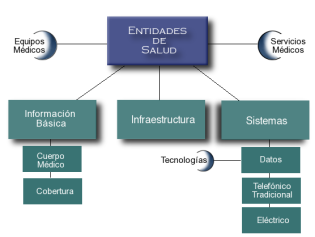
\includegraphics[width=80mm, height=52mm]{entidades.png}
 \caption{Arquitectura Básica de Prestador de Servicio de Salud}
\label{entidades}
\end{figure}

La información de estos nodos puede ser administrada por cada una de las entidades prestadoras de servicios de salud, de tal forma que se cree gradualmente un catálogo flexible para conocer el estado actual de las entidades y su potencialidad para ser parte en redes que presten servicios de salud a distancia usando TIC. De manera predeterminada las entidades se asocian a la arquitectura de red de la secretaría de Salud de Bogotá pero por medio del módulo denominado \textit{redes de atención} se puede crear cualquier prototipo de red jerárquica de atención \cite{yellowlees}.

\subsubsection{Tecnología de Interconexión} 
Nodos con datos de las tecnologías y protocolos de interconexión disponibles en las redes de acceso y transporte. Estas tecnologías se ordenan principalmente sobre el modelo de referencia OSI, pudiéndose crear  - desde el módulo de arquitecturas, cualquier otro tipo de modelo. En la actualidad se tiene como alternativa de clasificación el modelo TCP/IP. El conjunto de nodos de esta clase será una guía técnica que muestra la información de las capas físicas, de enlace y de red en formatos básicos- o de características generales; e intermedios - o de características técnicas.

El objetivo principal que se persigue es proveer a los analistas información para la revisión sistemática de las diferentes opciones que brindan los fabricantes de dispositivos y así proyectar redes que sean técnicamente viables. La información se estructura de acuerdo a indicadores cualitativos y cuantitativos que permiten evidenciar el carácter de interoperabilidad, impacto y permanencia de la tecnología en el mercado. 

\subsection{Equipo}
Nodos con datos técnicos sobre los diversos equipos con potencial uso en la telesalud - puede ser desde un equipo de resonancia magnética hasta un tablero interactivo. Posee atributos que son objetos de las clases Proveedor y Fabricante, así como la atributos de especificaciones técnicas, funcionales y físicas de los equipos.

\subsubsection{Operador de Telecomunicaciones}

\begin{figure}
 \centering
 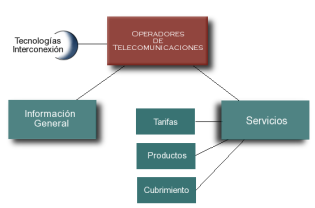
\includegraphics[width=80mm, height=52mm]{operadores.png}
 \caption{Arquitectura Básica de Operador de Telecomunicaciones}
 \label{operadores}
\end{figure}

Describe nodos de operadores de telecomunicaciones, figura \ref{operadores}, con énfasis en las características técnicas de los servicios que ofrecen, su cobertura y tarifas. Estos nodos brindan a los analistas información de operadores que permite determinar comparativas y evaluar las ventajas y desventajas entre diferentes opciones de interconexión. Este módulo se complementa con la información de dominio público que muestra el \textit{Sistema de Información Unificado para el sector de las Telecomunicaciones} mantenido por la Comisión Reguladora de Telecomunicaciones.

\subsection{Organización} 

Describe las características de organizaciones y grupos de investigación que trabajen en el área de la eSalud.  Estos nodos son claves para vislumbrar potencialidades de trabajo en grupo y de sistematizar experiencias adquiridas en los diferentes proyectos desarrollados en el área. 

\subsection{Servicios Médico} 
Este tipo de nodo cuya arquitectura se muestra en la figura \ref{servicios}, describe los servicios médicos y sus instancias componen una guía catalogada de los diferentes servicios y especialidades médicas disponibles. Se pone especial atención en la descripción detallada de los requerimientos técnicos y tecnológicos que requiere cada especialidad así como el perfil de los profesionales y entidades educativas de formación de especialistas. 

Se compone de clase que describen procedimientos, medicamentos, enfermedades, laboratorios, etc. 

\begin{figure}
 \centering
 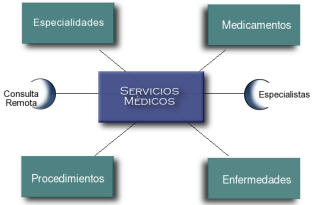
\includegraphics[width=80mm, height=60mm]{servicios.png}
 \caption{Arquitectura de Servicio Médico}
 \label{servicios}
\end{figure}

\subsection{Aplicaciones Federadas} 

Como patrón de desarrollo openSITEM integra a su arquitectura, soluciones de software libre o de código abierto, para proveer un ambiente integrado y aumentar sus prestaciones para implementar nuevos casos de uso. Entre las aplicaciones, mostradas en la figura \ref{aplicaciones_sitem}, que contribuyen a openSITEM se pueden citar:

\begin{description}

\item[Knowage] Suite de inteligencia analítica y de negocios.

\item[OpenProject] Sistema de gestión de proyectos.

\item[Alfresco] Sistema de Gestión Documental.

\item[Cesium] Visor geográfico 3D.

\item[WordPress] Sistema de Gestión de Contenido.

\item[SimpleSAML] Proveedor de identidad.

 \item[Moodle] Es un ambiente integrado de aplicaciones para la creación, organización, mantenimiento y seguimiento de cursos en línea. El fin primordial de sus herramientas es dar soporte a un marco de educación social constructivista.

\item[MapServer] Es una aplicación desarrollada en Python que proporciona al openSITEM los servicios básicos necesarios para la georeferenciación de la información.

\item[Sistema de Información Unificado del Sector de Telecomunicaciones] Conocido como SIUST, es un aplicativo Web desarrollado por la Comisión Reguladora de Telecomunicaciones que contiene información del sector de las telecomunicaciones en Colombia: “...información técnica de infraestructura, normatividad del sector, estadísticas comerciales e índices financieros de los prestadores de servicios y los indicadores de gestión del sector entre otros.” \footnote{Tomado del sitio web del SIUST. http://www.siust.gov.co/siust/}

La información, que es de acceso público, permite que openSITEM se nutra de ella para complementar y validar sus propias bases de datos en algunos subsistemas.

\item[Wikipedia] Quizás la fuente de información colaborativa más grande en Internet, debido a que sus contenidos son de uso libre, el SITEM se nutre de ellos y a su vez los complementa. A partir de información disponible se han editado más de 50 artículos en Wikipedia que tienen relación temática con el SITEM.

 \end{description}

\begin{figure}
 \centering
 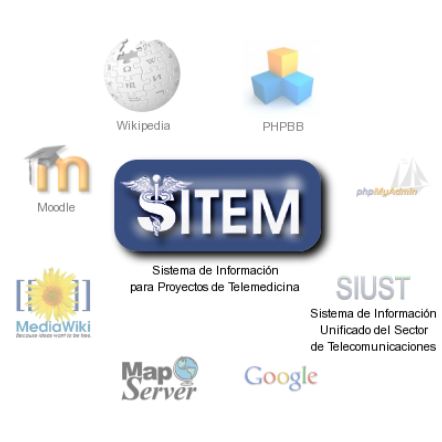
\includegraphics[width=156mm, height=156mm]{sitem_aplicaciones.png}
 \caption{Aplicaciones de Software Libre o Uso libre que complementan al SITEM}
 \label{aplicaciones_sitem}
\end{figure}

Es un principio del proyecto integrar otros productos de software libre promoviendo el uso de tales herramientas.